% @Author: Taha Bouhsine


%%%%%%%%%%%%%%%%%%%%%%%%%%%%
% CHAPTER                  %
%%%%%%%%%%%%%%%%%%%%%%%%%%%%
\setcounter{mtc}{6}

\chapter*{Introduction}
\label{chap:general_intorduction}
\minitoc
\markboth{\MakeUppercase{Introduction}}{}%
\addcontentsline{toc}{chapter}{Introduction}%
In recent years, crowdfunding has emerged as a revolutionary financing model that allows small entrepreneurs to raise funding in the early stages of their projects, particularly those that may otherwise struggle to obtain capital (Kuppuswamy and Bayus 2013; Belleflamme et al. 2014). Today, there are approximately 1250 active crowdfunding platforms across the world, which together channeled \$16.2 billion in 2014, representing a 167 \% increase from \$6.1 billion in 2013 (Massolution 2015). Having their project successfully funded is crucial to project creators as it provides not only initial funds for project development but also access to valuable future resources, and eventually turn their projects into successful entrepreneurial organizations (Mollick 2014). Previous research shows that only 45 \% of the projects on these platforms are successfully funded (Greenberg et al. 2013; Mollick 2014). As a result, identifying general antecedents of funding success (i.e., successfully funded) has been of great interest to researchers because it can provide insights to project creators to maximize their funding success (Greenberg et al. 2013; Xu et al. 2014).


One of the biggest topics discussed around the business community for the past few years is the idea of crowdfunding using an online platform. This is a great tool to use for building capital for a startup, funding growth for your company, or development of services or products to further your business.
New crowdfunding platforms and websites are popping up regularly to meet the needs of the expanding market, with plenty of room to benefit from the advantages of this technology by creating a crowdfunding platform.

\section*{Crowdfunding}
Crowdfunding is an increasingly popular alternative method of raising finance.
But what is crowdfunding? In this chapter, we will be explaining what crowdfunding is, how does it work, and what are the risks and rewards we face, and the latest Morocco's regulations on it.
\subsection*{Definition}
Crowdfunding is the practice of raising money from a large number of individuals for the purposes of financing a project, venture, business, or cause. Traditionally, crowdfunding has been carried out via subscriptions, benefit events, and door-to-door fundraising. However, today the term is typically associated with raising money through website platforms, which allows crowdfunding to reach a larger pool of potential funders.
\subsection*{History}
Crowdfunding has a long history with several roots. Books have been crowdfunded for centuries: authors and publishers would advertise book projects in praenumeration or subscription schemes. The book would be written and published if enough subscribers signaled their readiness to buy the book once it was out. The subscription business model is not exactly crowdfunding since the actual flow of money only begins with the arrival of the product. The list of subscribers has, though, the power to create the necessary confidence among investors that is needed to risk the publication.\\
War bonds are theoretically a form of crowdfunding military conflicts. London's mercantile community saved the Bank of England in the 1730s when customers demanded their pounds to be converted into gold - they supported the currency until confidence in the pound was restored, thus crowdfunded their own money. A clearer case of modern crowdfunding is Auguste Comte's scheme to issue notes for the public support of his further work as a philosopher. The "Première Circulaire Annuelle adressée par l\'auteur du Système de Philosophie Positive" was published on 14 March 1850, and several of these notes, blank and with sums have survived.\\
The cooperative movement of the 19th and 20th centuries is a broader precursor. It generated collective groups, such as community or interest-based groups, pooling subscribed funds to develop new concepts, products, and means of distribution and production, particularly in rural areas of Western Europe and North America. In 1885, when government sources failed to provide funding to build a monumental base for the Statue of Liberty, a newspaper-led campaign attracted small donations from 160,000 donors.\\
The late 19th century saw the creation of one of the world’s most recognizable landmarks with the gift of the Statue of Liberty by the French to the US. While the French paid for the construction and shipping of the statue it was down to the US to fund the base upon which it would stand.\\
With the statue ready to leave France, the Americans were still well short of the \$300,000 needed to build the base and erect the statue. Running short of time the American Committee (responsible for raising the funds) teamed up with newspaper owner Joseph Pulitzer to launch a campaign to invite citizens to donate even small amounts to help in the funding of a pedestal, offering donors miniature replicas of the statue in return.\\
This 19th-century crowdfunding campaign raised \$100,000 in mere of five months, contributed to one of the most popular attractions in the world and illustrated the financing power of a large crowd when tapped for funding.\\While the American Committee was lucky to have Mr Pulitzer and his paper to publicize their plea for donations, others wishing to access so many people would have had no such help. This, however, has changed in recent years with the rise of social media and the new ease with which communities can form and interact online.\\
Crowdfunding on the internet first gained popular and mainstream use in the arts and music communities.\\
The first noteworthy instance of online crowdfunding in the music industry was in 1997 when fans of the British rock band Marillion raised US\$60,000 in donations through an Internet campaign to underwrite an entire U.S. tour. The band subsequently used this method to fund their studio albums.\\
This built on the success of crowdfunding via magazines, such as the 1992 campaign by the Vegan Society that crowdfunded the production of the "Truth or Dairy" video documentary.
In the film industry, independent writer/director Mark Tapio Kines designed a website in 1997 for his then-unfinished first feature film Foreign Correspondents. By early 1999, he had raised more than US\$125,000 on the Internet from at least 25 fans, providing him with the funds to complete his film.\\
In 2002, the "Free Blender" campaign was an early software crowdfunding precursor.\\
The campaign aimed for open-sourcing the Blender 3D computer graphics software by collecting \$100,000 from the community while offering additional benefits for donating members.\\
The first company to engage in this business model was the U.S. website ArtistShare (2001).\\
As the model matured, more crowdfunding sites started to appear on the web such as Kiva (2005), IndieGoGo (2008), Kickstarter (2009), GoFundMe (2010), Microventures (2010), and YouCaring (2011).\\
The phenomenon of crowdfunding is older than the term "crowdfunding". According to wordspy.com, the earliest recorded use of the word was in August 2006.
\subsection*{ the Peer-To-Peer Lending Era }
Peer-to-peer lending, also abbreviated as P2P lending, is the practice of lending money to individuals or businesses through online services that match lenders with borrowers. Peer-to-peer lending companies often offer their services online, and attempt to operate with lower overhead and provide their services more cheaply than traditional financial institutions.[citation needed] As a result, lenders can earn higher returns compared to savings and investment products offered by banks, while borrowers can borrow money at lower interest rates,[1][2][3] even after the P2P lending company has taken a fee for providing the match-making platform and credit checking the borrower.


\subsection*{ Crowdfunding Types }
Crowdfunding facilitates the raising of capital for a variety of purposes, using numerous variations of the model. Below is a typology of how the operators in the market can potentially be segregated. The majority of platforms can be categorized under these four types, but there are several variations, such as hybrid models and those platforms that define themselves in a sectoral vertical rather than by the type of finance they provide.
\begin{enumerate}
      \item Donation Model:
            The donation model of crowdfunding is a means for charities, or those who raise money for social or charitable projects, to gather a community online and to enable them to donate to a project. While most established charities facilitate this through their own website, crowdfunding is popular for small organizations and people raising money for personal or specific charitable causes. Popular sites include Crowdrise and Causes.
      \item Lending Model:
            Crowdfunded lending is largely an evolution of the peer–to–peer model of lending, pioneered by firms such as Lendingclub and Zopa. Projects or businesses seeking debt apply through the platform uploading their pitch, with members of the crowd taking small chunks of the overall loan. Some platforms focused on social causes offer interest–free loans such as micro-lending site Kiva. Others operate more as an investment, where interest rates are decided either by those seeking the loan or using a market for loan parts, such as that used by UK platform FundingCircle.
      \item Reward Model:
            The most popular form of crowdfunding to date has been the reward model which has grown significantly in the funding of creative, social and entrepreneurial projects.
            The model allows people to contribute to projects and receive non–financial rewards in return, usually operating a tiered system where the more you donate the better the reward you receive. The model often closely resembles philanthropy with the donation far exceeding the monetary value of the reward or the reward costing the fundraiser little, such as experience or recognition–related rewards. For some projects the model is similar to a presale agreement.
            In these cases, entrepreneurs or artists crowdfund the production cost of their record, movie, game or product and allow the donors to be the first recipients once the production is complete. Popular platforms operating the reward model are Kickstarter and Indiegogo in the US and Peoplefund.it in the UK.
      \item Investment Model:
            The final type is the application of crowdfunding to investing for equity, or profit/revenue sharing in businesses or projects. This form of the model has been the slowest to grow due to regulatory restrictions that relate to this type of activity. Some European platforms have been pioneers of the equity crowdfunding model, allowing anyone to take a small stake in an unlisted or private business through crowdfunding. The most popular sites in offering this model are CrowdCube in the UK and Symbid in the Netherlands. Others such as
            Quirky offers a revenue or profit-sharing model allowing you to capitalize on the success of the projects you back.
\end{enumerate}


\subsection*{ How big is crowdfunding? }
In 2015, crowdfunding raised \$34 Billion worldwide (Source: Massolutions) and the total had doubled every year for the previous four years! Many crowdfunding campaigns are for quite small sums but some are very large. The model of crowdfunding which raised the most money is the lending model. In the UK crowdfunding in 2015 totaled £1,112 million and this figure is expected to continue to rise.


\subsection*{ Why is crowdfunding growing? }
Making a public call to fundraise from the crowd is not a new idea but crowdfunding as we now understand it has grown very quickly for a number of reasons since its emergence in the 1990s. These include:
\begin{enumerate}
      \item
            Technological developments : The emergence of wide and low-cost access to the internet and communication tools like social media mean it is easier and cheaper for us to reach out to much more widely dispersed and larger groups of people.
      \item
            Societal changes : These technical changes have also empowered us to take on new activities which were once controlled by gatekeepers. We can see this in the way people write and publish books, publish music, writing blogs, and the general sharing of our lives online. Crowdfunding is just the financial manifestation of this sense of empowerment and the ability to take “ownership” of a process. At the same time, we are also increasingly comfortable with transacting financially online be it shopping and e-commerce or checking our bank balances. This confidence to use money online is essential for the growth of crowdfunding.
      \item
            Economic factors : The other key factor in the extraordinary growth of crowdfunding is that after the financial crisis of 2008 access to funding has been more problematic and so people are exploring alternatives to the traditional sources. At the same time interest rates have fallen to historically low levels and so “retail investors” are looking for better places to put their investments and some crowdfunding campaigns seem to offer better returns than would be available on the high street.
\end{enumerate}

\subsection*{Principe }
The other important variation in crowdfunding is the distinction between what are known as the “Keep It All” and “All Or Nothing” models.\\
In a “Keep It All” campaign, you keep everything you raise regardless of whether you reach your target or not.\\
In an “All Or Nothing” campaign you only get to keep what you raise if you succeed in reaching your target.\\
Crowdfunding can be undertaken by both individuals and organizations.


%%%%% 
\subsection*{ Downsides of Crowdfunding}
\begin{enumerate}
      \item It is not easy – to be a success takes a lot of time and effort to carry out the continued promotion of your campaign.
      \item Many campaigns are unsuccessful and the successful ones take work, preparation and effort to make them happen – there is no guarantee of success but work, preparation and effort can increase the chances of success.
      \item It is also a very public process and so you must be prepared to be open and honest in a public arena and expect brickbats and bouquets in equal measure – it is important to accept that there may be public scrutiny of your project and prepare for this.
      \item Reputation considerations: there are a number of aspects to this, including your appearance on the platform in the first place. Might customers and others view it negatively? There are also significant expectations from investors if your crowdfunding campaign is successful. If it meets delays or runs into problems, the reputation of your company might become damaged. Finally, by putting your idea onto a crowdfunding platform before you’re ready to bring it to the wider market (i.e. before it’s fully developed and tested), you are leaving your company open to public criticism of your plans, idea, or business.
\end{enumerate}
%%%%%%%


\subsection*{ Benefits of Crowdfunding }
\begin{enumerate}
      \item It is a very accessible process which is open to all and can be carried out on your terms
      \item you decide on the amount you want to raise and the timescale to raise the funds.
      \item You are in control – the promotion and selling of the project is the responsibility of your group.
      \item It can bring much more than money – it can attract new people and support (nonfinancial) to your group.
      \item What money it does bring can be very different from a traditional investment – funds raised through crowdfunding are unrestricted and can be used for all elements of your project.
      \item It can be quick – as you are in control you are able to work quickly to start raising funds.
      \item You will also produce a very valuable asset for you or your organization as you run a campaign and that “crowd asset” can be a very useful and enduring resource – people who support your project are also likely to support your group.
      \item It’s a quick and easy way to get a lot of exposure for your brand and for your new idea or initiative
      \item You can engage directly with investors who could also become your customers
      \item There is a low barrier to entry – often much lower than with other forms of investment
      \item It’s an easy way to get feedback on your idea
\end{enumerate}


\subsection*{ What makes crowdfunding different from other funding? }
Crowdfunding reaches widely by using technology and reduces the size of funding each individual contributor has to come up with. This means that more people can take part.
Making it easy for a wider group of people to support a business or project introduces a wider range of motivations for people to back a campaign. This means that there is a range of reasons why people might support you, and not simply for a financial return.
The idea of many small contributions making a difference (as opposed to a small number of large contributions) is a concept underpinning lots of online activities which have disrupted traditional industries and it is called “The Long Tail”.
Because the process of crowdfunding is a very public one and involves many people it can, and does, bring many more advantages than simply money. It can be a powerful campaigning tool, it can build networks, validate an idea, build awareness and many other things, all of which can be very valuable and useful. A good crowdfunding campaign will recognize and target these additionalities.
For some entrepreneurial projects, it has the advantage of accelerating the process of setting up a business by allowing the entrepreneur to run in parallel a series of processes like market research, publicity and marketing and fundraising, which have often traditionally been seen as sequential.



\subsection*{ Motivation And Rewards }



\subsection*{ Crowdfunding Actors }
In crowdfunding there is two main actors, the project owner that created the fundraiser, and the actor that provide the funds.
\begin{enumerate}
      \item Creator
      \item Funder
\end{enumerate}

\subsection*{ Existent Platforms }
Non-Profit:
\begin{enumerate}
      \item
            Fundly: This is probably the best known of the non-profit crowdfunding sites. This platform charges a fee for all campaigns and a small transaction fee for processing. It offers a customizable donation page, with an integrated mobile experience. You can use multiple media formats to promote your cause as well as blogging.
      \item
            Salsa: This p2p platform offers branded marketing materials for every supporter and customizes messages as well. This is a fully integrated system with Salsa CRM. So, if you already use that, software data is transferred easily.
      \item
            Soapbox Engage: This is a social change platform that offers not only the ability to create cause for donation but allows you to create forms, petitions, and events to further your cause.
      \item
            Bonfire: is a crowdfunding platform that allows you to create custom t-shirts to raise money for your projects. You create the t-shirt and then build a custom web page to market and use as a landing spot to drive your social media marketing campaigns.
\end{enumerate}
Business:
\begin{enumerate}
      \item
            Kickstarter: This is a crowdfunding platform that allows you to market potential products or businesses for investors to donate to. You create a custom page for your book, game, or any other creative project and then set a goal and start building funds. Each project will set up designated donations that have rewards attached to them.
      \item
            Indigogo: This is a great sight for startups and creatives that uses similar methods to Kickstarter. You set up a custom page and goals and market your campaign. They have integrated systems to help with the fulfillment of delivery, mobile management, perk options, etc.
      \item
            Seedrs: This crowdfunding platform uses equity investing to raise funds for small businesses and startups. It has three options to invest whether equity, funds or convertible donations and allows other investors a discount in the future.
      \item
            Crowdcube: This platform offers you the chance to invest in business and causes via an easy-to-use website. Creating campaigns via your own customizable page, you will have access to analytics and social media campaigns to help promote your project.
\end{enumerate}




\subsection*{ Crowdfunding In Morocco }
Expected since April 2018, the examination of the so-called «collaborative financing» bill is finally starting in Morocco. In the latter case, for management companies that want to propose capital investment, it will be necessary to obtain a visa from the Moroccan Capital Market Authority . The platforms must have a minimum capital of \$31,000 and the collaborative finance companies that will manage them must have a risk prevention and reduction policy.
A few researchers in the Economic field started a study [\cite{crowdMorocco}], to understand the future of crowdfunding in Morocco, they started a survey with a total of 200 participants over the internet. Surprisingly,  The majority of respondents 96\% do not even know what the word crowdfunding means, and of 5\% left most respondents that know about crowdfunding plan to have their projects with a percentage of 62\%, while 5\% answered I do not know against 33\% do not want to have their projects. However, according to the distribution by the labor force, they found that this majority consists mainly of the unemployed and students, while more than half of the workers do not want to have their projects. For those who want to have their projects, it is mainly the lack of funding , and the lack of idea and the risk of failure that prevents them, so crowdfunding can fill this gap is becoming an alternative to financing projects or even a compliment. Finally, they found that the majority who want to start their project and who have financing problems for a percentage of 55.5\% are interested in crowdfunding to launch or develop their projects, however, the lack of information on this system is the first cause for those who are not interested in this new mode of financing, which is normal.


\begin{figure}[!ht]
      \center
      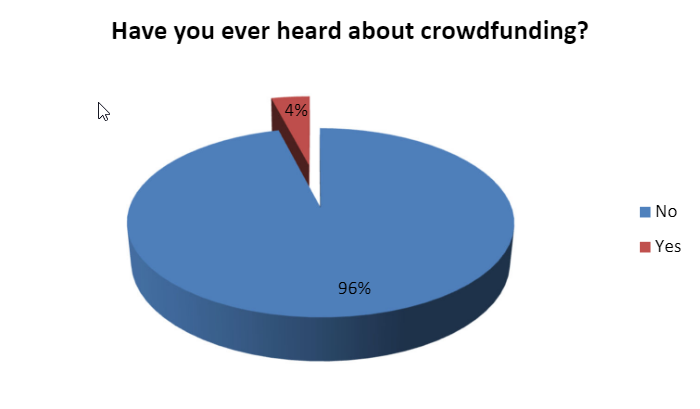
\includegraphics[scale=0.60]{assets/heardCrowd.png}
      \caption{ Have you ever heard of crowdfunding? }
      \label{fig:heardCrowd}
\end{figure}

\begin{figure}[!ht]
      \center
      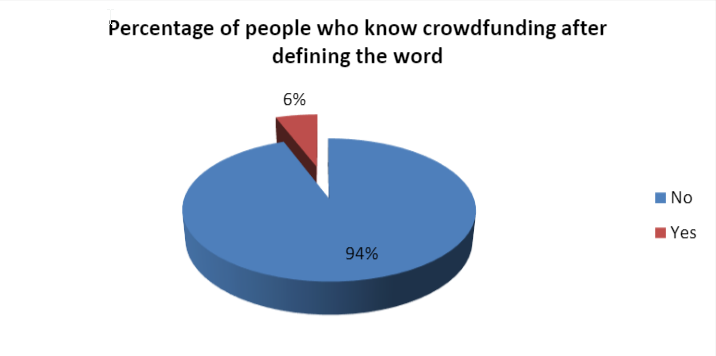
\includegraphics[scale=0.60]{assets/knowCrowd.png}
      \caption{Do you know what crowdfunding is? After explaining the meaning of crowdfunding}
      \label{fig:knowCrowd}
\end{figure}

\begin{figure}[!ht]
      \center
      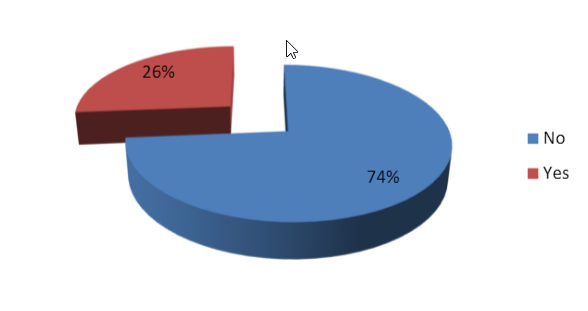
\includegraphics[scale=0.60]{assets/knowPlatform.png}
      \caption{Do you already know a crowdfunding platform?}
      \label{fig:knowPlatform}
\end{figure}

\begin{figure}[!ht]
      \center
      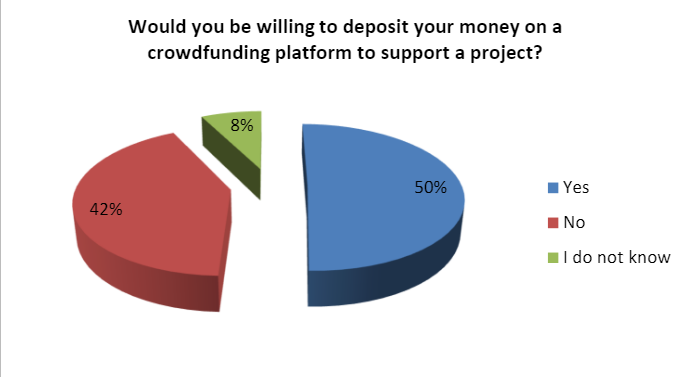
\includegraphics[scale=0.60]{assets/willing.png}
      \caption{Would you be willing to deposit your money on a crowdfunding platform to support a project?}
      \label{fig:willing}
\end{figure}


